% Options for packages loaded elsewhere
\PassOptionsToPackage{unicode}{hyperref}
\PassOptionsToPackage{hyphens}{url}
\documentclass[
  12pt,
]{article}
\usepackage{xcolor}
\usepackage[margin=1in]{geometry}
\usepackage{amsmath,amssymb}
\setcounter{secnumdepth}{-\maxdimen} % remove section numbering
\usepackage{iftex}
\ifPDFTeX
  \usepackage[T1]{fontenc}
  \usepackage[utf8]{inputenc}
  \usepackage{textcomp} % provide euro and other symbols
\else % if luatex or xetex
  \usepackage{unicode-math} % this also loads fontspec
  \defaultfontfeatures{Scale=MatchLowercase}
  \defaultfontfeatures[\rmfamily]{Ligatures=TeX,Scale=1}
\fi
\usepackage{lmodern}
\ifPDFTeX\else
  % xetex/luatex font selection
  \setmainfont[]{Times New Roman}
\fi
% Use upquote if available, for straight quotes in verbatim environments
\IfFileExists{upquote.sty}{\usepackage{upquote}}{}
\IfFileExists{microtype.sty}{% use microtype if available
  \usepackage[]{microtype}
  \UseMicrotypeSet[protrusion]{basicmath} % disable protrusion for tt fonts
}{}
\makeatletter
\@ifundefined{KOMAClassName}{% if non-KOMA class
  \IfFileExists{parskip.sty}{%
    \usepackage{parskip}
  }{% else
    \setlength{\parindent}{0pt}
    \setlength{\parskip}{6pt plus 2pt minus 1pt}}
}{% if KOMA class
  \KOMAoptions{parskip=half}}
\makeatother
\usepackage{graphicx}
\makeatletter
\newsavebox\pandoc@box
\newcommand*\pandocbounded[1]{% scales image to fit in text height/width
  \sbox\pandoc@box{#1}%
  \Gscale@div\@tempa{\textheight}{\dimexpr\ht\pandoc@box+\dp\pandoc@box\relax}%
  \Gscale@div\@tempb{\linewidth}{\wd\pandoc@box}%
  \ifdim\@tempb\p@<\@tempa\p@\let\@tempa\@tempb\fi% select the smaller of both
  \ifdim\@tempa\p@<\p@\scalebox{\@tempa}{\usebox\pandoc@box}%
  \else\usebox{\pandoc@box}%
  \fi%
}
% Set default figure placement to htbp
\def\fps@figure{htbp}
\makeatother
\setlength{\emergencystretch}{3em} % prevent overfull lines
\providecommand{\tightlist}{%
  \setlength{\itemsep}{0pt}\setlength{\parskip}{0pt}}
\usepackage{xcolor}
\usepackage{float}
\usepackage{colortbl}
\usepackage[table]{xcolor}
\usepackage{graphicx}
\usepackage{lscape}
\usepackage{tikz}
\usepackage{amsmath}
\usepackage{tcolorbox}
\usepackage{fancyhdr}
\usepackage{lipsum}
\setlength{\headheight}{15.35403pt}
\addtolength{\topmargin}{-2.5pt}
\pagestyle{fancy}
\fancyhead[L]{\textcolor{purple}{M2 SSD - BIOSTAT}}
\fancyhead[C]{\textcolor{purple}{Support Vector Machine \textbf{-} HAX907X}}
\fancyhead[R]{\textcolor{purple}{2025 \textbf{-} 2026}}
\fancyfoot[C]{\thepage}
\renewcommand{\contentsname}{Table des matières}
\usepackage{bookmark}
\IfFileExists{xurl.sty}{\usepackage{xurl}}{} % add URL line breaks if available
\urlstyle{same}
\hypersetup{
  hidelinks,
  pdfcreator={LaTeX via pandoc}}

\author{}
\date{\vspace{-2.5em}}

\begin{document}

\begin{titlepage}
\definecolor{umcolor}{RGB}{85, 37, 130}

\begin{center}

% Logo en haut

\includegraphics[width=0.3\linewidth]{vis/logo/logo_m.png}\\[1.5cm]

% Université et département
{\Large \textsc{Université de Montpellier}}\\[0.2cm]
{\large Département de Mathématiques Appliquées}\\[1.5cm]

% Encadré du titre
\tcbset{colback=blue!20, colframe=red, width=\textwidth, arc=3mm, boxrule=0.8mm}
\begin{tcolorbox}
    \centering
    {\huge \bfseries TP3 : Support Vector Machine}\\[0.3cm]
    {\large \textit{Apprentissage Statistique — HAX907X}}
\end{tcolorbox}

\vfill

% Auteur
\begin{flushright}
    \textbf{Réalisé par :}\\
    ATTOUMANI Ibrahim
\end{flushright}

\vfill

% Bas de page

\includegraphics[width=0.25\linewidth]{vis/logo/ssd.png}\\[0.3cm]
{\Large Année Universitaire 2025 -- 2026}

\end{center}
\end{titlepage}

\thispagestyle{empty}
\definecolor{navy}{RGB}{11, 11, 69}
\definecolor{picker}{RGB}{235, 153, 30}

\newpage
\thispagestyle{empty}
\tableofcontents
\newpage

\section{\texorpdfstring{\textcolor{red}{1. Introduction}}{}}\label{section}

Les \textbf{SVM} (Support Vector Machines), introduits par Vapnik, sont
des méthodes de classification très utilisées, en particulier pour la
classification binaire. Elles reposent sur la recherche d'une règle de
décision linéaire sous la forme d'un \textbf{hyperplan séparateur}. Pour
traiter des problèmes plus complexes, cette recherche est effectuée non
pas directement dans l'espace des données initiales, mais dans un
\textbf{espace de caractéristiques} de grande dimension, obtenu grâce à
une transformation non linéaire.

L'objectif de ce TP est d'appliquer les SVM sur des données réelles et
simulées à l'aide de la librairie \texttt{scikit-learn} (qui s'appuie
sur \texttt{libsvm}). Nous apprendrons également à ajuster les
\textbf{hyperparamètres} et le \textbf{choix du noyau} afin de mieux
contrôler la flexibilité du modèle. \newpage

\section{\texorpdfstring{\textcolor{red}{2. Classification sur les donnée Iris}}{}}\label{section-1}

Dans cette section, nous allons mettre en œuvre un \textbf{SVM linéaire}
afin de distinguer les classes \textbf{1 et 2} du jeu de données
\textit{iris}. Pour simplifier le problème, seules les
\textbf{deux premières variables} seront utilisées. Nous conserverons la
moitié des données pour l'\textbf{apprentissage} et l'autre moitié pour
le \textbf{test}, afin d'évaluer la capacité du modèle à bien
généraliser.

\subsection{\texorpdfstring{\textcolor{blue}{2.1. SVM linéaire : discrimination entre les classes 1 et 2 d’Iris}}{}}\label{section-2}

Ici nous allons sélectionner les classes 1 et 2 du dataset
\textit{iris}, puis conserver uniquement les deux premières variables
(longueur et largeur des sépales) afin de simplifier la visualisation et
la classification.

\begin{figure}[H]
    \centering
    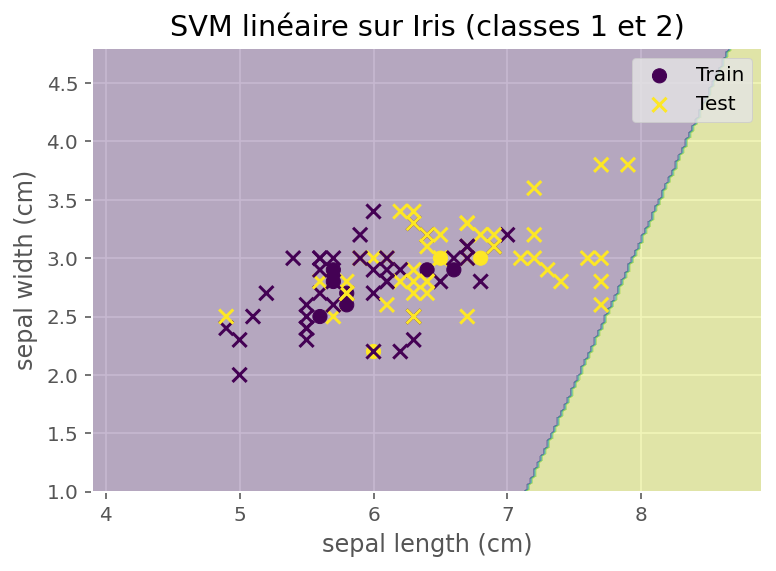
\includegraphics[width=0.8\textwidth]{vis/classif_90test_10train.png}
    \caption{SVM linéaire avec 90\% des données réservées au test}
    \label{fig:svm_iris_90test_10train}
\end{figure}

Ci-dessus, on a dédiées 90\% des données pour le test, ce qui ne laisse
qu'environ 10\% pour l'entraînement (soit seulement 10 points). Avec si
peu d'exemples, le SVM ne dispose pas d'assez d'informations pour bien
apprendre. On a alors que la frontière de décision est très
approximative et la précision sur le test chute à \textbf{0.48}, proche
du hasard.

En utilisant 40\% des données pour le test, nous obtenons une précision
de 7\%. Comparée à la \textbf{figure 1}, la frontière de décision sépare
mieux les points, bien que quelques erreurs de prédiction subsistent. La
\textbf{figure 2} ci-dessous illustre cette visualisation.

\begin{figure}[H]
    \centering
    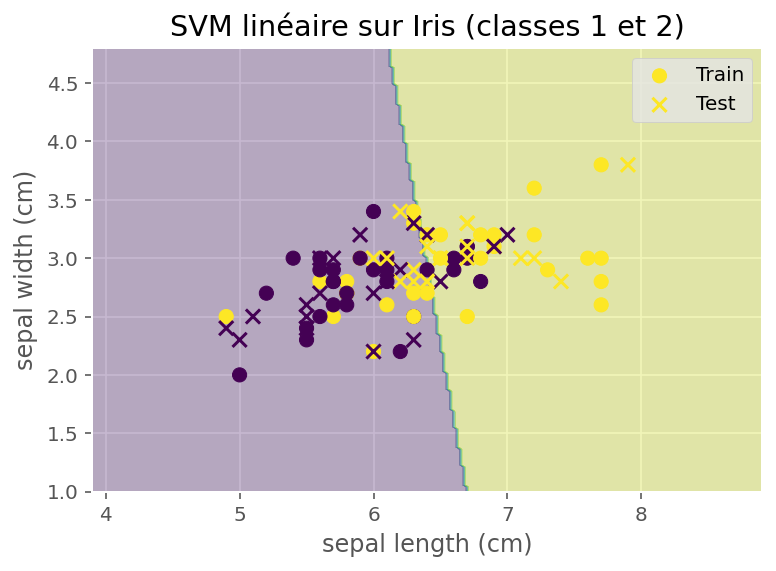
\includegraphics[width=0.65\textwidth]{vis/classif_40test_60train.png}
    \caption{SVM linéaire avec 40\% des données réservées au test}
    \label{fig:svm_iris_40test_60train}
\end{figure}

\subsection{\texorpdfstring{\textcolor{blue}{2.2. SVM polynomial : discrimination entre les classes 1 et 2 d’Iris}}{}}\label{section-3}

Dans cette section, nous entraînons un SVM avec noyau polynomial pour
discriminer les classes 1 et 2 d'Iris. Ce noyau permet de modéliser des
frontières de décision non linéaires, plus flexibles que celles du SVM
linéaire. Nous comparerons ensuite ses performances et sa frontière de
décision avec celles du SVM linéaire présenté précédemment.

\begin{figure}[H]
    \centering
    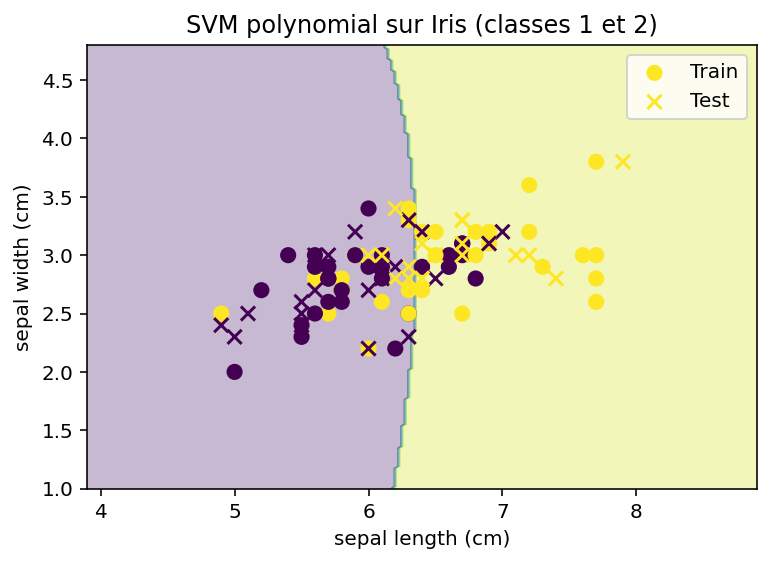
\includegraphics[width=0.65\textwidth]{vis/classif_poly_40test_60train.png}
    \caption{SVM polynomial avec 40\% des données réservées au test}
    \label{fig:svm_poly_iris_40test_60train}
\end{figure}

À présent, nous comparons la classification linéaire à la classification
polynomiale. Cette dernière ajuste mieux la frontière de décision, avec
une précision de 0.75 sur le jeu de test. Comme pour la classification
linéaire, 40\% des données ont été utilisées pour l'évaluation.

\begin{figure}[H]
    \centering
    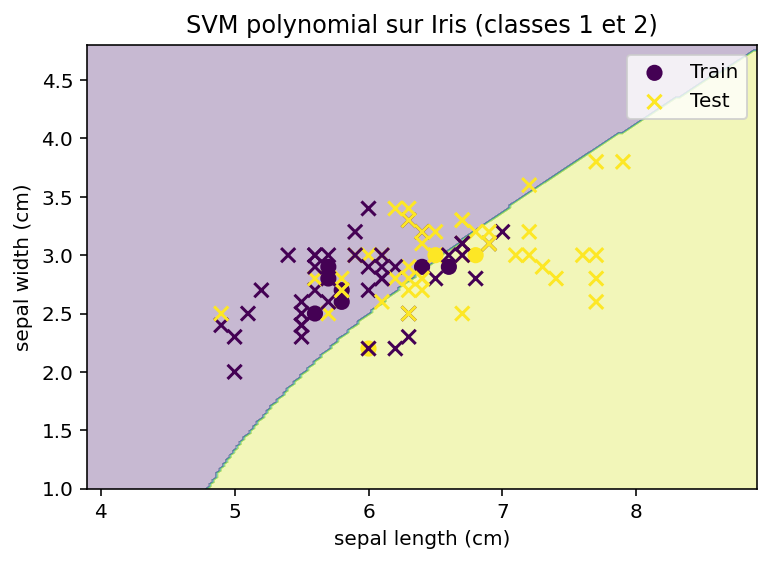
\includegraphics[width=0.65\textwidth]{vis/classif_poly_90test_10train.png}
    \caption{SVM polynomial avec 90\% des données réservées au test}
    \label{fig:svm_poly_iris_90test_10train}
\end{figure}

Nous avons testé deux modèles SVM (linéaire et polynomial) sur les
classes 1 et 2 de l'iris, en utilisant les caractéristiques
\textit{sepal length} et \textit{sepal width}.

Avec une grande proportion de données en test (90\%), les deux modèles
donnent de faibles scores, mais le SVM polynomial s'adapte mieux grâce à
une frontière de décision non linéaire.

Avec une répartition plus équilibrée (60\% train / 40\% test), les
performances s'améliorent. Le SVM polynomial reste légèrement meilleur,
car il capture mieux la séparation non linéaire entre les classes.

\subsection{\texorpdfstring{\textcolor{blue}{2.3. SVM GUI: données simulées déséquilibré}}{}}\label{section-4}

Cette application
\textcolor{red}{svm\_gui.py}(\textcolor{blue}{https://scikit-learn.org/1.2/auto\_examples/applications/svm\_gui.html})
permet en temps réel d'évaluer l'impact du noyaux et du paramètre de
régularisation \(C\).

Dans ce qui suit, nous allons générer un jeu de données très
déséquilibré avec beaucoup plus de points dans une classe que dans
l'autre. Ensuite, nous utiliserons un noyau linéaire tout en réduisant
le paramètre \(C\) et observerons le résultat.

Lorsque l'on diminue la valeur du paramètre \(C=0,001\), le SVM devient
plus tolérant aux erreurs. La frontière de décision se simplifie et ne
cherche plus à bien séparer toutes les classes.

Dans un jeu de données très déséquilibré (90\% vs 10\%), cela entraîne
un fort biais vers la classe majoritaire. La classe minoritaire est
alors mal reconnue, voire ignorée. La figure ci-dessous illustre la
frontière de décision d'un problème déséquilibré:

\begin{figure}[H]
    \centering
    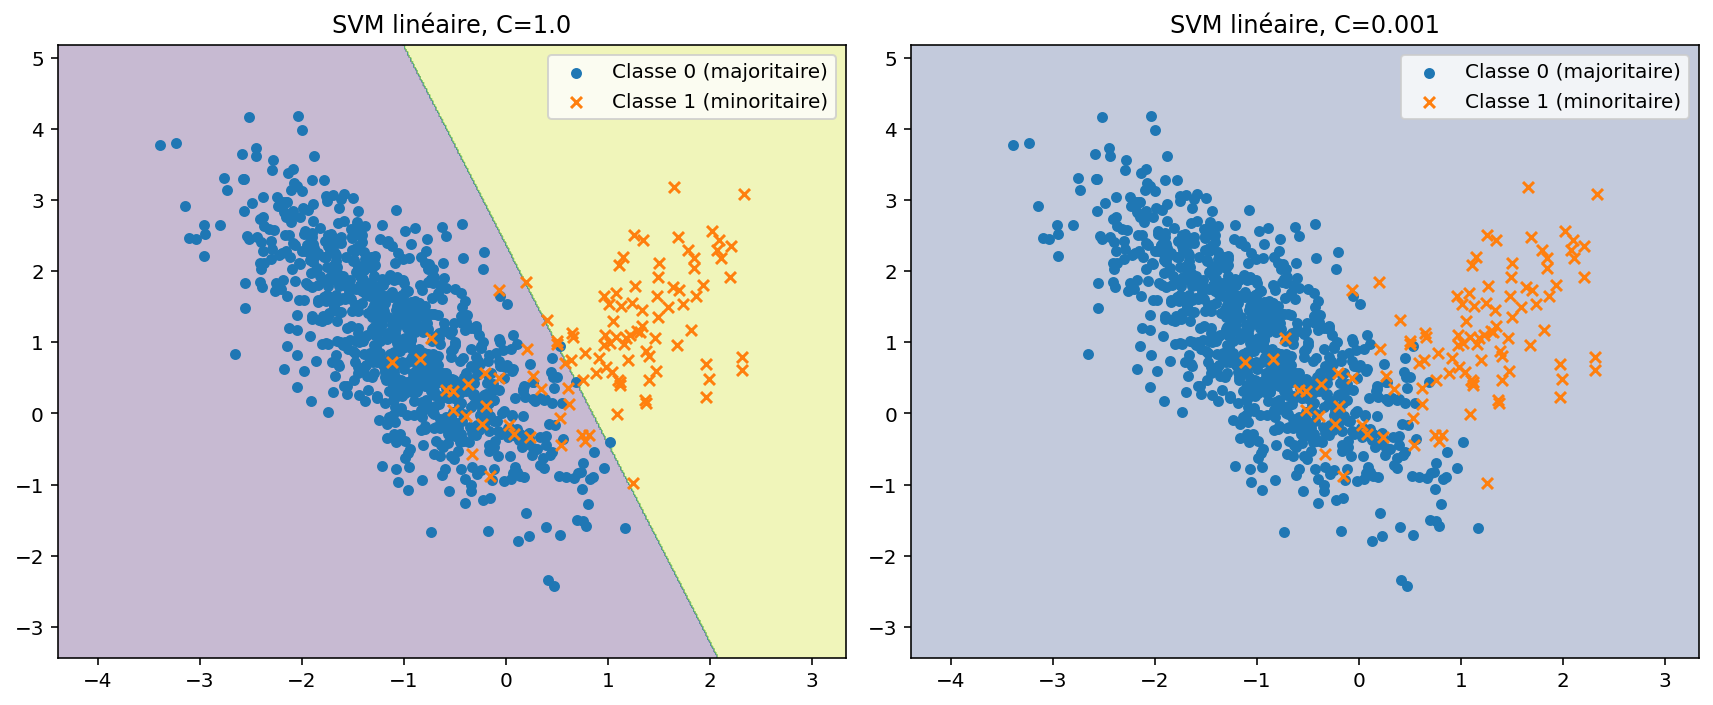
\includegraphics[width=0.9\textwidth]{vis/classif_simul_cpetit.png}
    \caption{SVM linéaire avec $C = 0.001$ sur données déséquilibrées.}
    \label{fig:simule_c_petit}
\end{figure}

Pour résoudre le problème de données déséquilibrées, nous pouvons
utiliser l'option \texttt{class\_weight="balanced"} dans le SVM. Cette
approche permet d'ajouter une correction par pondération, en donnant
davantage de poids à la classe minoritaire afin d'éviter qu'elle soit
ignorée par le modèle.

L'illustration de ce phénomène, avec et sans correction par pondération,
est présentée en annexe.

\section{\texorpdfstring{\textcolor{red}{3. Classification de visage}}{}}\label{section-5}

\newpage

\section{\texorpdfstring{\textcolor{red}{Annexe}}{}}\label{section-6}

Ce code génère un jeu de données binaire fortement déséquilibré (90,\%
vs 10,\%). Deux modèles SVM linéaires sont ensuite entraînés : l'un sans
pondération et l'autre avec l'option \texttt{class\_weight="balanced"}.
Enfin, la frontière de décision de chaque modèle est tracée afin de
comparer l'effet de la pondération sur la classe minoritaire.

Le code complet utilisé pour générer les comparaisons de frontières de
décision est disponible sur GitHub à l'adresse suivante :

\textcolor{blue}{\url{https://github.com/atttoum8643f/tp_svm/blob/main/code_py/corr_ponderation.py}}

\begin{figure}[H]
    \centering
    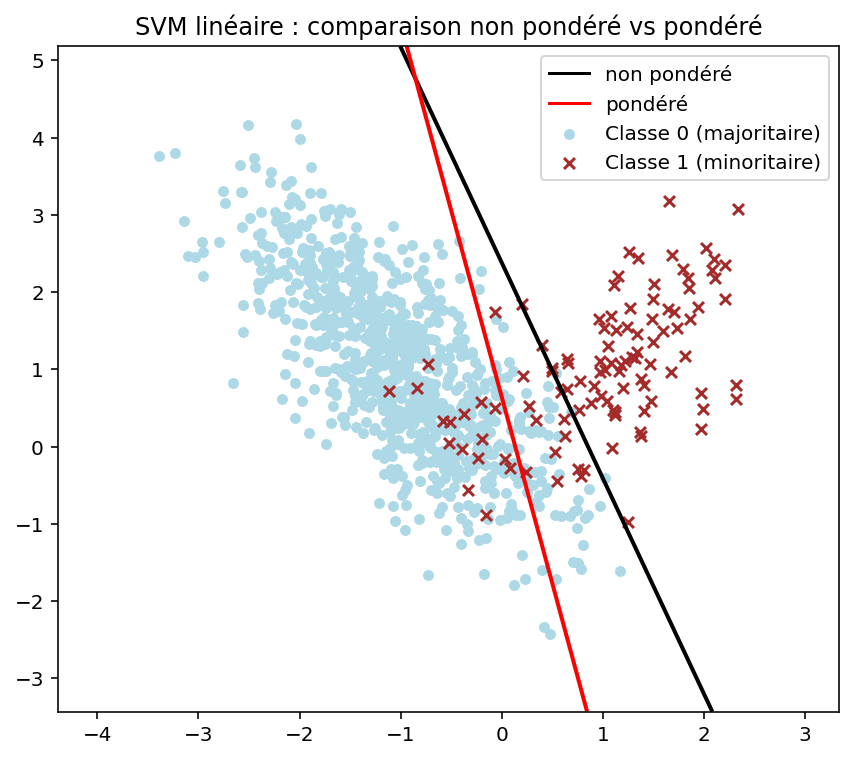
\includegraphics[width=0.75\textwidth]{vis/pond.png}
    \caption{Frontière de décision d’un SVM linéaire avec et sans correction par pondération}
    \label{fig:avec_sans_pondération}
\end{figure}

\begin{thebibliography}{9}

\bibitem{scikit-learn}
scikit-learn developers.  
\textit{Support Vector Machines — scikit-learn documentation}.  
\url{http://scikit-learn.org/stable/modules/svm.html}.  
Consulté le 24 septembre 2025.

\bibitem{wiki-en}
Wikipedia.  
\textit{Support vector machine}.  
\url{http://en.wikipedia.org/wiki/Support_vector_machine}.  
Consulté le 24 septembre 2025.

\bibitem{wiki-fr}
Wikipédia.  
\textit{Machine à vecteurs de support}.  
\url{http://fr.wikipedia.org/wiki/Machine_%C3%A0_vecteurs_de_support}.  %C3%A0_vecteurs_de_support}.  %A0_vecteurs_de_support}.  
Consulté le 24 septembre 2025.

\end{thebibliography}

\end{document}
